\item  O alvo é um disco circular fino de \SI{5}{\kilogram} que pode girar livremente em torno do eixo $z$. Uma bala de \SI{25}{\gram}, viajando a \SI{600}{\meter/\second}, acerta o alvo em $A$ e fica embutida nele. Determine a velocidade angular do alvo após o impacto. Inicialmente, ele está em repouso.

\import{../answers}{answer-12}

\vspace{-.4cm}
\begin{flushright}
	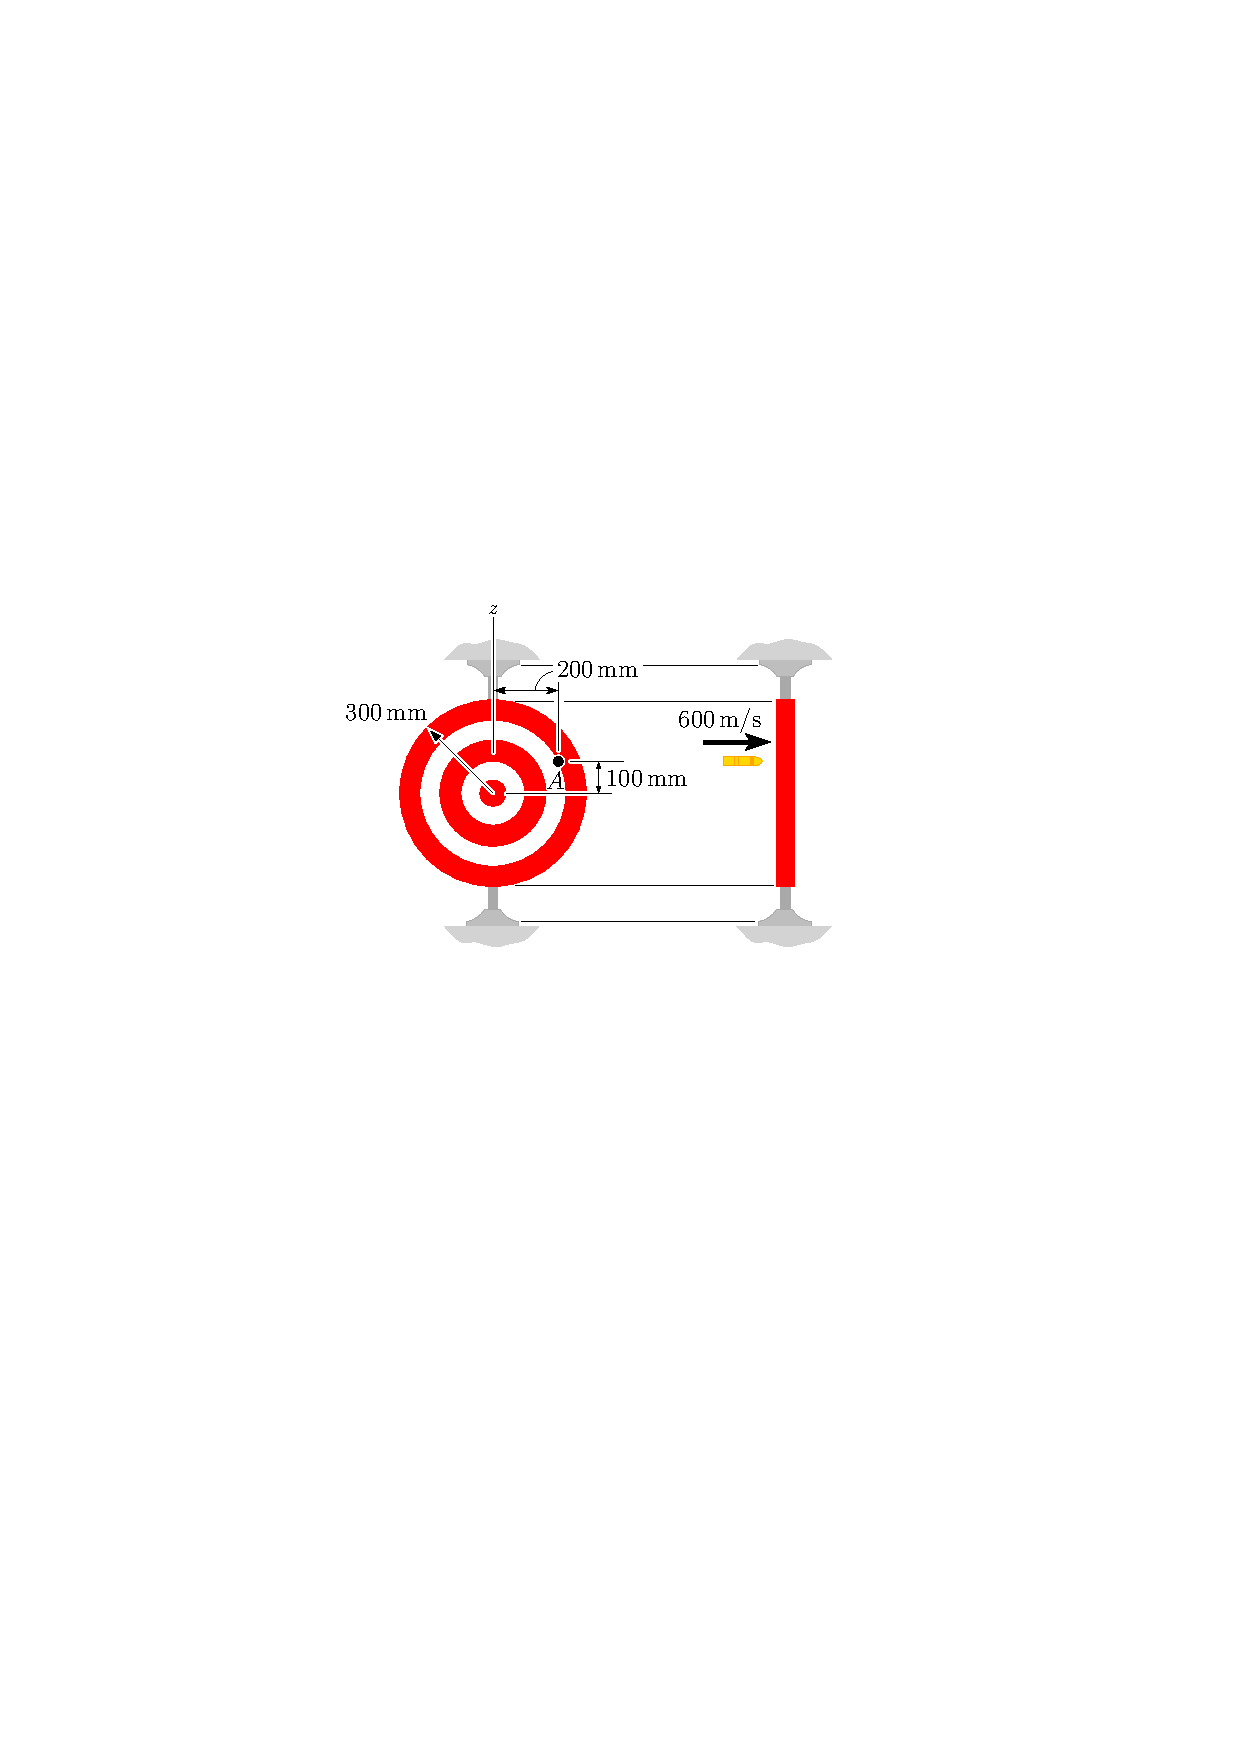
\includegraphics[scale=1.1]{../../images/draw_8}
\end{flushright}
